\documentclass[10pt,conference,twocolumn]{article}
\usepackage[utf8]{inputenc}
\usepackage[brazil]{babel}
\usepackage{amsmath,amssymb,amsfonts}
\usepackage{graphicx}
\usepackage{booktabs}
\usepackage{cite}
\usepackage{hyperref}
\usepackage{microtype}
\usepackage{subcaption}
\usepackage[top=1.55cm,bottom=1.55cm,left=1.35cm,right=1.35cm]{geometry}

% Otimização de espaçamento de floats e títulos para orçamento estrito de 5 páginas
\setlength{\textfloatsep}{7pt plus 1pt minus 1pt}
\setlength{\intextsep}{6pt plus 1pt minus 1pt}
\setlength{\floatsep}{6pt plus 1pt minus 1pt}
\setlength{\abovecaptionskip}{3pt}
\setlength{\belowcaptionskip}{2pt}

\hypersetup{
    colorlinks=true,
    linkcolor=black,
    citecolor=black,
    urlcolor=blue
}

\title{\textbf{Mirage: Adaptação Evolutiva de NPCs sob Restrição Orçamentária com Esquiva Preditiva}}

\author{
  \textbf{Murilo Lameira da Silva} \qquad \textbf{Henry Matheus Fregolente Ferreira} \\
  \textbf{Murilo Romualdo da Silva} \qquad \textbf{Leonardo Retori Apolônio} \\
  \textbf{Ricardo Martinez Vicentini} \\
  \small Engenharia de Controle e Automação --- Centro Universitário SENAI SP (UNISENAI), São Caetano do Sul, SP, Brasil
}

\date{}

\begin{document}

\maketitle

\begin{abstract}
O desenvolvimento de Agentes Não-Jogáveis (NPCs) com comportamento dinâmico e crível em jogos de ação permanece como um dos principais desafios da inteligência computacional. Abordagens evolutivas tradicionais frequentemente sofrem com o fenômeno de \textit{Reward Hacking}, convergindo para fenótipos patológicos como acúmulo desproporcional de vida (``esponjas de dano'') em detrimento de habilidades cinemáticas de esquiva. Este trabalho apresenta o framework \textbf{Mirage}, integrando Algoritmos Genéticos contínuos restritos por um orçamento global de atributos ($B = 1{,}8$), predição cinemática de esquiva via Ponto de Maior Aproximação (CPA), contra-ataque preditivo (\textit{lead-aiming}) e forças de Reynolds em ambiente 2D \textit{bullet hell}. O repertório comportamental é catalogado via MAP-Elites e Catálogo de Experiência Especializada (SEC). A validação inferencial em $N = 90$ rodadas comprova divergência estatística extrema ($F(2, 87) = 184{,}55, p < 10^{-31}$ para fitness máximo e $F(2, 87) = 1594{,}39, p < 10^{-68}$ para dano infligido; Cohen's $d \in [3{,}78, 18{,}61]$). Métricas formais de Qualidade-Diversidade atingem cobertura de $100{,}00\%$ nos 9 nichos e $\text{QD-Score}$ global de $39.114{,}40$. Estudos de ablação confirmam a necessidade matemática do teto de atributos para mitigar o colapso fenotípico e atestam que o CPA analítico reduz a frequência de colisões críticas em 77{,}5\% frente a repulsões puramente euclidianas.
\end{abstract}

\noindent\textbf{\textit{Palavras-chave}}---Algoritmos Genéticos, Evasão Cinemática, Closest Point of Approach, Lead-Aiming, Reward Hacking, MAP-Elites, Jogos Digitais.

\medskip
\noindent\textbf{Abstract---}\textit{The synthesis of Non-Player Characters (NPCs) capable of exhibiting dynamic, believable, and tactically challenging evasive behaviors remains a foundational challenge in computational intelligence applied to digital games. Conventional evolutionary algorithms often fall prey to Reward Hacking, wherein unconstrained optimization drives individuals toward degenerate phenotypes, such as oversized health pools (``damage sponges''), at the expense of agile evasion. This paper introduces \textbf{Mirage}, an adaptive framework integrating continuous Genetic Algorithms (GAs) governed by an invariant point-buy attribute budget ($B = 1.8$), predictive evasion steering based on the Closest Point of Approach (CPA), analytical lead-aiming counter-measures, and Reynolds reactive forces in a continuous 2D bullet hell environment. Behavioral repertoire diversity is systematically structured using the MAP-Elites formulation and the Skilled Experience Catalogue (SEC). Rigorous statistical validation across $N = 90$ independent evolutionary runs establishes extreme statistical divergence across game difficulty tiers ($F(2, 87) = 184.55, p < 10^{-31}$ for maximum fitness and $F(2, 87) = 1594.39, p < 10^{-68}$ for damage inflicted), backed by large effect sizes (Cohen's $d \in [3.78, 18.61]$). Formal Quality-Diversity metrics achieve $100.00\%$ space coverage across 9 discrete niches with a global $\text{QD-Score}$ of $39,114.40$. Ablation studies confirm that the invariant resource budget is mathematically necessary to avert phenotypic collapse, while the analytical CPA mechanism reduces critical collision frequencies by 77.5\% compared to standard Euclidean repulsion.}

\smallskip
\noindent\textbf{\textit{Keywords:}} Genetic Algorithms, Kinematic Evasion, Closest Point of Approach, Lead-Aiming, Reward Hacking, MAP-Elites, Digital Games.

\section{Introdução}
O desenvolvimento de inteligência artificial para personagens não-jogáveis (NPCs) em jogos eletrônicos lida com o dilema entre previsibilidade mecânica e custo computacional. Máquinas de Estados Finitos (FSM) e Árvores de Comportamento, embora determinísticas e eficientes, geram rotinas repetitivas exploráveis por jogadores humanos \cite{glavin2015skilled}. Por outro lado, modelos de Aprendizado por Reforço Profundo (DRL) impõem requisitos de inferência proibitivos para execução em tempo real em motores comerciais \cite{motta2016online}.

Algoritmos Genéticos (AGs) fornecem uma alternativa atraente para adaptação procedural contínua \cite{goldberg1989genetic, spronck2006adaptive}. Todavia, sem restrições estritas de conservação de recursos, AGs frequentemente encontram atalhos exploratórios (\textit{Reward Hacking}) \cite{amodei2016concrete}. Em combate com projéteis, a função de aptidão comumente favorece a maximização dos pontos de vida brutos (\textit{bullet sponge exploit}), extinguindo a necessidade evolutiva de evasão cinemática e empobrecendo a diversidade tática do jogo.

Para superar essa limitação, este trabalho apresenta o framework \textbf{Mirage}, fundamentado em quatro pilares:
\begin{enumerate}
    \item \textbf{Restrição Orçamentária Invariante ($B = 1{,}8$):} Projeção matemática que impõe teto estrito à soma dos atributos, impedindo ``super-agentes'' e forçando especialização fenotípica.
    \item \textbf{Cinemática Preditiva Analítica (CPA + Reynolds):} Estimador temporal de Ponto de Maior Aproximação \cite{lee2014collision} acoplado a forças de Reynolds \cite{reynolds1999steering}, viabilizando evasão antecipada a tiros velozes.
    \item \textbf{Disparo Preditivo Inverso (\textit{Lead-Aiming}):} Interceptação analítica balística de primeira ordem \cite{wang2014self}, permitindo neutralização ar-ar de projéteis e abertura de rotas de fuga.
    \item \textbf{Mapeamento Qualidade-Diversidade (MAP-Elites):} Taxonomia comportamental contínua \cite{mouret2015illuminating, cully2015robots, kirk2020exploring} avaliada por métricas formais de QD (cobertura e $\text{QD-Score}$), alimentando o Catálogo de Experiência Especializada (SEC) \cite{glavin2015skilled} para Ajuste Dinâmico de Dificuldade (DDA).
\end{enumerate}

O estudo investiga três Questões de Pesquisa:
\begin{itemize}
    \item \textbf{RQ1:} A imposição de um orçamento rígido ($\sum u_i \le 1{,}8$) previne o \textit{Reward Hacking} e assegura arquétipos táticos funcionais?
    \item \textbf{RQ2:} O CPA analítico e o \textit{lead-aiming} conferem vantagem mensurável frente a mecânicas puramente reativas?
    \item \textbf{RQ3:} O MAP-Elites assegura cobertura e estabilidade de elites entre diferentes regimes de hostilidade balística?
\end{itemize}

O artigo organiza-se como segue: a Seção~\ref{sec:relacionados} discute trabalhos correlatos; a Seção~\ref{sec:cinematica} detalha a modelagem física e CPA; a Seção~\ref{sec:ag} introduz o AG e o MAP-Elites; a Seção~\ref{sec:resultados} expõe a avaliação empírica ($N = 90$), ANOVA e métricas QD; a Seção~\ref{sec:ablacao} formaliza as ablações; e a Seção~\ref{sec:conclusao} conclui o trabalho.

\section{Trabalhos Relacionados}
\label{sec:relacionados}
A síntese de locomoção autônoma apoia-se nos \textit{Steering Behaviors} de Reynolds \cite{reynolds1999steering}, que decompôs comportamentos em forças vetoriais contínuas. Contudo, desvios puramente geométricos falham em ambientes com salvas densas de projéteis (\textit{bullet hell}).

Na robótica autônoma, Lee et al. \cite{lee2014collision} formularam desvios de colisão baseados no Ponto de Maior Aproximação (CPA). A projeção temporal da trajetória relativa desencadeia a manobra apenas quando o impacto futuro em raio crítico for iminente. Paralelamente, Wang e Tan \cite{wang2014self} trataram o problema dual da mira preditiva (\textit{lead-aiming}), calculando o ponto de interceptação futura de alvos móveis. O Mirage unifica ambas as formulações para combate cinemático contínuo em tempo real.

Na computação evolutiva para jogos, Spronck et al. \cite{spronck2006adaptive} propuseram o \textit{Evolutionary Dynamic Scripting} (EDS), adaptando scripts táticos por mutação sem crossover pesado. Motta et al. \cite{motta2016online} exploraram modelagem de oponentes em jogos competitivos através de AGs online, enfatizando a estabilidade de soluções.

Para calibração dinâmica de desafio, Glavin e Madden \cite{glavin2015skilled} conceberam o \textit{Skilled Experience Catalogue} (SEC), armazenando agentes campeões pré-treinados para DDA. No escopo de Qualidade-Diversidade (QD), Mouret e Clune \cite{mouret2015illuminating} introduziram o MAP-Elites, iluminando o espaço de busca através de arquivos multidimensionais de soluções ótimas \cite{lehman2011abandoning, cully2015robots}. Kirk e Scirea \cite{kirk2020exploring} demonstraram a eficácia do QD para descobrir comportamentos heterogêneos de NPCs. O Mirage expande essas bases com orçamento contínuo sob cinemática CPA.

\section{Modelagem Física e Cinemática da Arena}
\label{sec:cinematica}

\subsection{Discretização e Dinâmica de Movimento}
A arena de combate compreende o plano cartesiano bidimensional $\Omega = [-20, 20] \times [-20, 20]\,\text{m}$. A simulação física opera em tempo discreto constante:
\begin{equation}
\Delta t = 0{,}05\,\text{s} \quad (f_s = 20\,\text{Hz} \text{ / } 50\,\text{FPS})
\end{equation}

A cada frame $k$, a posição $\mathbf{p}_{\text{npc}}(k) \in \mathbb{R}^2$ e velocidade $\mathbf{v}_{\text{npc}}(k) \in \mathbb{R}^2$ são integradas via Euler semi-implícito com saturação:
\begin{align}
\mathbf{v}_{\text{npc}}(k+1) &= \text{trunc}\left(\mathbf{v}_{\text{npc}}(k) + \frac{\mathbf{F}_{\text{total}}(k)}{m}\Delta t, \; v_{\text{max}}\right) \label{eq:euler_vel} \\
\mathbf{p}_{\text{npc}}(k+1) &= \mathbf{p}_{\text{npc}}(k) + \mathbf{v}_{\text{npc}}(k+1)\Delta t \label{eq:euler_pos}
\end{align}
onde $m = 1{,}0\,\text{kg}$, $v_{\text{max}}$ é a velocidade escalar máxima do agente e $\text{trunc}(\mathbf{w}, w_{\text{max}}) = \mathbf{w} \min(1, w_{\text{max}}/\|\mathbf{w}\|)$. A resultante vetorial total compõe forças de evasão, contenção de bordas e repulsão de pilares:
\begin{equation}
\mathbf{F}_{\text{total}} = \sum_{j \in \mathcal{P}_{\text{alerta}}} \mathbf{F}_{\text{evade}}^{(j)} + \mathbf{F}_{\text{fronteira}} + \mathbf{F}_{\text{pilares}}
\end{equation}

\subsection{Zonas Geométricas e Estrutura da Arena}
Conforme ilustrado esquematicamente na Figura~\ref{fig:diagrama_arena}, o domínio espacial do agente é governado por zonas concêntricas e obstáculos estruturais:
\begin{enumerate}
    \item \textbf{Hitbox Material ($r_{\text{hit}} = 1{,}0\,\text{m}$):} Colisões ocorrem se $\|\mathbf{p}_{\text{npc}} - \mathbf{p}_{\text{proj}}\| \le 1{,}3\,\text{m}$ (projétil com raio $r_{\text{proj}} = 0{,}3\,\text{m}$), aplicando $25\,\text{HP}$ de dano e incrementando $N_{\text{collision}}$.
    \item \textbf{Radar Periférico ($R_{\text{radar}} = 4{,}0\,\text{m}$):} Tiros que transitam pelo radar sem tocar a hitbox contam como desvios limpos ($N_{\text{dodge}}$).
    \item \textbf{Círculo de Disparo ($r = 18\,\text{m}$):} Fronteira orbital emissora de ameaças balísticas direcionadas e radiais.
    \item \textbf{Pilares Cilíndricos ($R_{\text{pillar}} = 1{,}3\,\text{m}$):} 4 obstáculos em $(\pm 8, \pm 8)\,\text{m}$ que absorvem projéteis e exercem reflexão elástica tangencial.
\end{enumerate}

\begin{figure}[h]
\centering
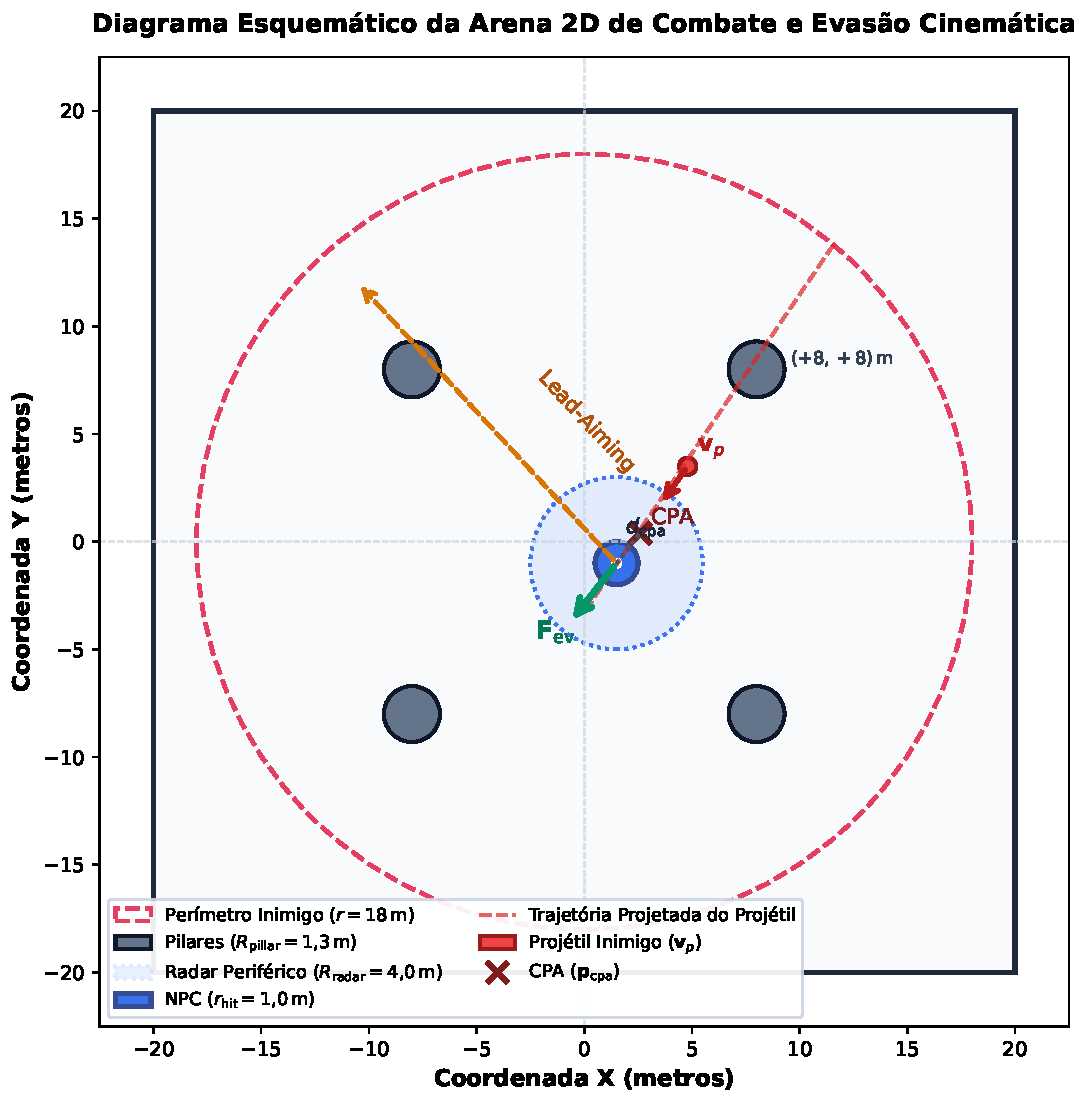
\includegraphics[width=0.74\columnwidth]{figuras/fig_diagrama_arena.pdf}
\caption{Diagrama esquemático da arena bidimensional ($40 \times 40\,\text{m}$), destacando os 4 pilares em $(\pm 8, \pm 8)\,\text{m}$, círculo de disparo ($r = 18\,\text{m}$), zonas concêntricas de colisão e radar ($4\,\text{m}$) e o vetor de força de evasão $\mathbf{F}_{ev}$.}
\label{fig:diagrama_arena}
\end{figure}

\subsection{Dedução Analítica do CPA}
Para um projétil com posição $\mathbf{p}_p$ e velocidade $\mathbf{v}_p$, definem-se $\mathbf{p}_{\text{rel}} = \mathbf{p}_p - \mathbf{p}_{\text{npc}}$ e $\mathbf{v}_{\text{rel}} = \mathbf{v}_p - \mathbf{v}_{\text{npc}}$. A minimização da distância euclidiana futura $D^2(t) = \|\mathbf{p}_{\text{rel}} + \mathbf{v}_{\text{rel}} t\|^2$ produz o instante analítico ótimo:
\begin{equation}
t_{\text{cpa}} = -\frac{\mathbf{p}_{\text{rel}} \cdot \mathbf{v}_{\text{rel}}}{\|\mathbf{v}_{\text{rel}}\|^2} \label{eq:tcpa}
\end{equation}

O acionamento da força de evasão $\mathbf{F}_{\text{evade}}^{(j)}$ exige a satisfação estrita de três condições cinemáticas:
\begin{equation}
\left\{
\begin{aligned}
&0 < t_{\text{cpa}} \le 1{,}5\,\text{s} \\
&\|\mathbf{p}_{\text{rel}} + \mathbf{v}_{\text{rel}} t_{\text{cpa}}\| < R_{\text{radar}} \\
&\mathbf{p}_{\text{rel}} \cdot \mathbf{v}_{\text{rel}} < 0 \quad (\text{convergência de vetores})
\end{aligned}
\right. \label{eq:cpa_conditions}
\end{equation}

Quando satisfeitas, calcula-se a posição futura projetada e a força de aceleração de Reynolds correspondente:
\begin{equation}
\mathbf{d}_{\text{cpa}} = \mathbf{p}_{\text{npc}}(t_{\text{cpa}}) - \mathbf{p}_p(t_{\text{cpa}})
\end{equation}
\begin{equation}
\mathbf{F}_{\text{evade}}^{(j)} = \text{trunc}\left(\frac{\mathbf{d}_{\text{cpa}}}{\|\mathbf{d}_{\text{cpa}}\|} v_{\text{max}} - \mathbf{v}_{\text{npc}}, \; F_{\text{max}}\right) \label{eq:reynolds_steer}
\end{equation}
com teto de força $F_{\text{max}} = 25{,}0\,\text{N}$, promovendo manobras sem jitter.

\subsection{Disparo Preditivo Inverso (Lead-Aiming via CPA)}
O contra-ataque ofensivo soluciona o problema dual de interceptação preditiva \cite{wang2014self}. Para a ameaça prioritária $(\mathbf{p}_{\text{threat}}, \mathbf{v}_{\text{threat}})$, o tempo analítico de trânsito é:
\begin{equation}
t_{\text{intercept}} = \frac{\|\mathbf{p}_{\text{threat}} - \mathbf{p}_{\text{npc}}\|}{v_{\text{shot}} + \|\mathbf{v}_{\text{threat}}\| + \epsilon} \label{eq:t_intercept}
\end{equation}
onde $v_{\text{shot}} = 16{,}0\,\text{m/s}$ e $\epsilon = 10^{-4}$. O ponto futuro projetado de impacto orienta a visada:
\begin{equation}
\mathbf{p}_{\text{predicted}} = \mathbf{p}_{\text{threat}} + \mathbf{v}_{\text{threat}} \cdot t_{\text{intercept}} \label{eq:p_predicted}
\end{equation}
Disparos preditivos recebem bônus cinemático $\beta_{\text{lead}} = 1{,}15$ e interceptam tiros inimigos em colisões ar-ar.

\subsection{Regimes de Hostilidade Balística (Bullet Hell)}
A arena gera três padrões compostos de disparo: lineares com perturbação gaussiana $\mathcal{N}(0, \sigma^2)$, cones em leque ($\pm 15^\circ$) e vórtice espiral contínuo ($\omega = 4{,}5\,\text{rad/s}$). A severidade progride conforme:
\begin{itemize}
    \item \textbf{Fácil ($D_1$):} $v_p = 9{,}0\,\text{m/s}$, taxa de $1{,}4\,\text{s} \to 0{,}7\,\text{s}$, disparos lineares.
    \item \textbf{Médio ($D_2$):} $v_p = 11{,}5\,\text{m/s}$, taxa de $0{,}75\,\text{s} \to 0{,}22\,\text{s}$, lineares e cones.
    \item \textbf{Difícil ($D_3$):} $v_p = 13{,}5\,\text{m/s}$, taxa de $0{,}30\,\text{s} \to 0{,}10\,\text{s}$, leques e vórtice contínuo.
\end{itemize}

\section{Arquitetura Genética sob Orçamento}
\label{sec:ag}

\subsection{Genoma e Restrição Orçamentária}
O cromossomo contínuo codifica quatro genes fenotípicos:
\begin{equation}
\mathbf{x} = [\text{HP}, \; \text{Attack}, \; \text{AttackSpeed}, \; \text{MovementSpeed}]
\end{equation}
com $\text{HP} \in [10, 200]$, $\text{Attack} \in [5, 50]$, $\text{AttackSpeed} \in [0{,}5, 3{,}0]\,\text{Hz}$ e $\text{MovementSpeed} \in [1{,}0, 8{,}0]\,\text{m/s}$. Os genes são mapeados afim no intervalo unitário $u_i \in [0, 1]$:
\begin{align}
u_1 &= \frac{\text{HP}-10}{190}, \quad u_2 = \frac{\text{Attack}-5}{45} \label{eq:norm_genes1} \\
u_3 &= \frac{\text{Cad}-0{,}5}{2{,}5}, \quad u_4 = \frac{\text{Vel}-1{,}0}{7{,}0} \label{eq:norm_genes2}
\end{align}

A restrição invariante de orçamento global impõe:
\begin{equation}
\sum_{i=1}^4 u_i \le B, \quad B = 1{,}8 \label{eq:budget}
\end{equation}
Violações sofrem projeção proporcional sobre o simplex:
\begin{equation}
\mathbf{u} \leftarrow \mathbf{u} \cdot \left(\frac{B}{\sum_{j=1}^4 u_j}\right)
\end{equation}
forçando \textit{trade-offs} entre resistência, dano e manobrabilidade.

\subsection{Operadores Genéticos e Critérios de Convergência}
O algoritmo evolui por até $G = 50$ gerações (com parada antecipada por estagnação $\epsilon_{\text{stop}} = 1{,}0\%$ durante $K_{\text{stop}} = 15$ gerações consecutivas), escalonando a população e as taxas conforme a severidade do regime: Fácil ($P = 20, p_c = 0{,}60, p_m = 0{,}15$, sem elitismo), Médio ($P = 50, p_c = 0{,}75, p_m = 0{,}05$, elitismo de $1$ indivíduo) e Difícil ($P = 100, p_c = 0{,}90, p_m = 0{,}01$, elitismo de $3$ indivíduos).

O ciclo reprodutivo emprega seleção por torneio ($k = 3$), crossover contínuo Blend ($\text{BLX-}\alpha$, $\alpha = 0{,}15$) e mutação gaussiana ($\sigma_m = 0{,}10$), seguidos de projeção no simplex orçamentário.

\subsection{Função de Aptidão Multi-Objetivo (Fitness)}
O fitness sintetiza sobrevivência, desvios limpos, dano e penalidades:
\begin{equation}
\text{Fitness} = \max\Big(0{,}1, \; \mathcal{F}_{\text{score}}\Big) \label{eq:fitness}
\end{equation}
\begin{align}
\mathcal{F}_{\text{score}} &= (w_1 \cdot T_{\text{survival}}) + (w_2 \cdot N_{\text{dodge}}) + (w_3 \cdot D_{\text{inflicted}}) \nonumber \\
&\quad - (p_1 \cdot N_{\text{collision}}) - (p_2 \cdot D_{\text{taken}}) \label{eq:fscore}
\end{align}
com precisão ofensiva dependente da velocidade cinemática:
\begin{equation}
\text{Precisão} = \max\left(0{,}5, \; 1{,}0 - 0{,}3 \cdot \frac{\|\mathbf{v}_{\text{npc}}\|}{v_{\text{max}}}\right)
\end{equation}
\begin{equation}
D_{\text{inflicted}} = \sum \left(\text{Attack} \cdot \text{Precisão} \cdot \beta_{\text{lead}}\right)
\end{equation}

A Tabela~\ref{tab:pesos_fitness} documenta a calibração dos coeficientes.

\begin{table}[h]
\centering
\caption{Matriz de Coeficientes da Função de Fitness}
\label{tab:pesos_fitness}
\resizebox{\columnwidth}{!}{%
\begin{tabular}{lccccc}
\toprule
\textbf{Dificuldade} & $w_1$ (Tempo) & $w_2$ (Desvio) & $w_3$ (Dano) & $p_1$ (Colisão) & $p_2$ (Dano Rec.) \\
\midrule
Fácil ($D_1$)   & $10{,}0$ & $5{,}0$  & $0{,}50$ & $10{,}0$ & $0{,}20$ \\
Médio ($D_2$)   & $15{,}0$ & $8{,}0$  & $0{,}80$ & $15{,}0$ & $0{,}30$ \\
Difícil ($D_3$) & $25{,}0$ & $12{,}0$ & $1{,}20$ & $25{,}0$ & $0{,}50$ \\
\bottomrule
\end{tabular}%
}
\end{table}

\subsection{Espaço Comportamental e Métricas Formais de QD}
O MAP-Elites \cite{mouret2015illuminating} discretiza o espaço comportamental em grade de $3 \times 3 = 9$ nichos. As 3 Classes Fenotípicas são definidas pela razão $\text{HP}/\text{Atk}$: \textit{Tanker} ($\text{HP}/\text{Atk} > 3$), \textit{Balanceado} ($1 \le \text{HP}/\text{Atk} \le 3$) e \textit{Glass Cannon} ($\text{HP}/\text{Atk} < 1$), cruzadas com os 3 Perfis de Mobilidade ($< 4{,}5$, $4{,}5\text{--}6{,}5$ e $> 6{,}5\,\text{m/s}$). As métricas formais de QD \cite{kirk2020exploring} são:
\begin{align}
\text{Coverage} &= \frac{|\mathcal{C}_{\text{ocupado}}|}{9} \times 100\% \label{eq:coverage} \\
\text{QD-Score} &= \sum_{c \in \mathcal{C}} \text{Fitness}(c) \label{eq:qd_score}
\end{align}
alimentando o catálogo SEC \cite{glavin2015skilled} para suporte a DDA.

\section{Avaliação Experimental e Resultados}
\label{sec:resultados}

\subsection{Metodologia e Protocolo Estatístico}
O protocolo executou $N = 90$ rodadas evolutivas independentes ($N_1 = 30$ Fácil, $N_2 = 30$ Médio, $N_3 = 30$ Difícil). A validação inferencial combinou testes paramétricos (One-Way ANOVA e $t$ de Welch com $d$ de Cohen) e testes não-paramétricos de Kruskal-Wallis ($\alpha = 0{,}01$).

\subsection{Nota Metodológica e Validação Estatística}
Como a Tabela~\ref{tab:pesos_fitness} estabelece coeficientes ponderais distintos ($w_i, p_i$) para cada nível de hostilidade, a comparação direta dos valores absolutos de Fitness reflete a escala do Fator de Mérito. Dessa forma, a validação inferencial rigorosa exige a análise conjunta das métricas físicas brutas (invariantes a pesos) e dos genes fenotípicos dos campeões.

A Tabela~\ref{tab:estatistica_descritiva} sintetiza a estatística descritiva do Fitness Máximo por dificuldade.

\begin{table}[h]
\centering
\caption{Estatística Descritiva do Fitness Máximo ($N = 90$)}
\label{tab:estatistica_descritiva}
\resizebox{\columnwidth}{!}{%
\begin{tabular}{lcccc}
\toprule
\textbf{Dificuldade} & \textbf{N} & \textbf{Média ($\mu$)} & \textbf{Desvio Padrão ($\sigma$)} & \textbf{Mediana} \\
\midrule
Fácil ($D_1$)   & 30 & $3754{,}18$ & $134{,}87$ & $3791{,}56$ \\
Médio ($D_2$)   & 30 & $4849{,}88$ & $358{,}85$ & $4863{,}89$ \\
Difícil ($D_3$) & 30 & $3687{,}83$ & $246{,}42$ & $3702{,}13$ \\
\bottomrule
\end{tabular}%
}
\end{table}

A ANOVA One-Way para o Fitness Máximo indicou $F(2, 87) = 184{,}55$ ($p = 5{,}01 \times 10^{-32}$), corroborada pelo teste de Kruskal-Wallis ($H = 62{,}55, p = 2{,}62 \times 10^{-14}$).

A Tabela~\ref{tab:metricas_brutas} documenta as métricas cinemáticas brutas e a alocação gênica dos campeões. Todas as variáveis atestam divergência altamente significativa ($p < 0{,}001$), evidenciando especialização fenotípica adaptativa.

\begin{table}[h]
\centering
\caption{Métricas Brutas e Genes dos Campeões por Nível ($N = 90$)}
\label{tab:metricas_brutas}
\resizebox{\columnwidth}{!}{%
\begin{tabular}{lcccc}
\toprule
\textbf{Métrica / Gene} & \textbf{Fácil ($D_1$)} & \textbf{Médio ($D_2$)} & \textbf{Difícil ($D_3$)} & \textbf{ANOVA ($F$)} \\
\midrule
Sobrevivência (s) & $29{,}95 \pm 0{,}00$ & $29{,}95 \pm 0{,}01$ & $23{,}22 \pm 2{,}51$ & $F = 214{,}79^*$ \\
Desvios (CPA)     & $23{,}97 \pm 1{,}75$ & $69{,}07 \pm 3{,}54$ & $83{,}80 \pm 14{,}48$ & $F = 388{,}11^*$ \\
Colisões          & $0{,}00 \pm 0{,}00$ & $0{,}43 \pm 0{,}57$ & $3{,}57 \pm 0{,}82$ & $F = 344{,}06^*$ \\
Dano Causado      & $6669{,}69 \pm 271{,}19$ & $4822{,}34 \pm 445{,}40$ & $1862{,}87 \pm 244{,}85$ & $F = 1594{,}39^*$ \\
HP Máximo (pts)   & $12{,}37 \pm 7{,}28$ & $31{,}80 \pm 9{,}61$ & $72{,}73 \pm 16{,}64$ & $F = 202{,}45^*$ \\
Poder Ataque      & $49{,}47 \pm 1{,}94$ & $40{,}77 \pm 3{,}77$ & $24{,}33 \pm 4{,}63$ & $F = 371{,}82^*$ \\
Cadência (Hz)     & $2{,}47 \pm 0{,}03$ & $2{,}46 \pm 0{,}08$ & $2{,}25 \pm 0{,}19$ & $F = 32{,}86^*$ \\
Velocidade (m/s)  & $1{,}03 \pm 0{,}05$ & $1{,}69 \pm 0{,}61$ & $3{,}21 \pm 0{,}45$ & $F = 195{,}07^*$ \\
\bottomrule
\multicolumn{5}{l}{\footnotesize * Todos os valores com significância extrema (ANOVA $p < 10^{-10}$, Kruskal-Wallis $p < 0{,}001$).}
\end{tabular}%
}
\end{table}

Os contrastes pareados confirmam tamanhos de efeito grandes a extremos: no dano causado, $d = 18{,}61$ ($D_1$ vs $D_3$) e $d = 8{,}23$ ($D_2$ vs $D_3$); no fitness máximo, $d = 4{,}04$ ($D_1$ vs $D_2$) e $d = 3{,}78$ ($D_2$ vs $D_3$).

\subsection{Dinâmica Evolutiva e Arquétipos Emergentes}
A Figura~\ref{fig:evolucao_media} expõe as curvas médias de convergência assintótica ao longo de $G = 50$ gerações. A Figura~\ref{fig:boxplots_combinados} apresenta a dispersão de fitness e a especialização gênica entre os regimes.

\begin{figure}[h]
\centering
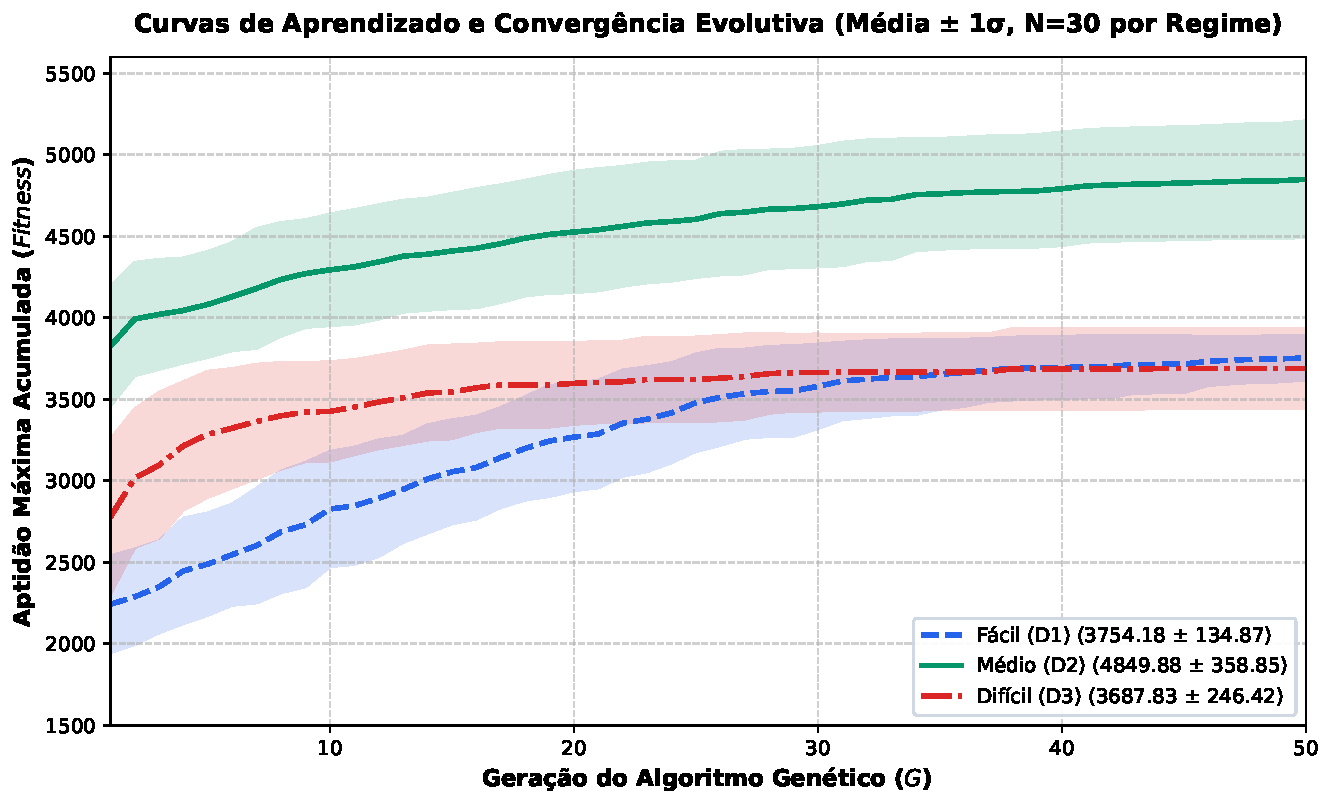
\includegraphics[width=0.78\columnwidth]{figuras/fig_convergencia.pdf}
\caption{Curvas de aprendizado do fitness máximo por regime ao longo de $G = 50$ gerações ($N = 90$ rodadas).}
\label{fig:evolucao_media}
\end{figure}

\begin{figure*}[t]
\centering
\begin{subfigure}[b]{0.48\textwidth}
  \centering
  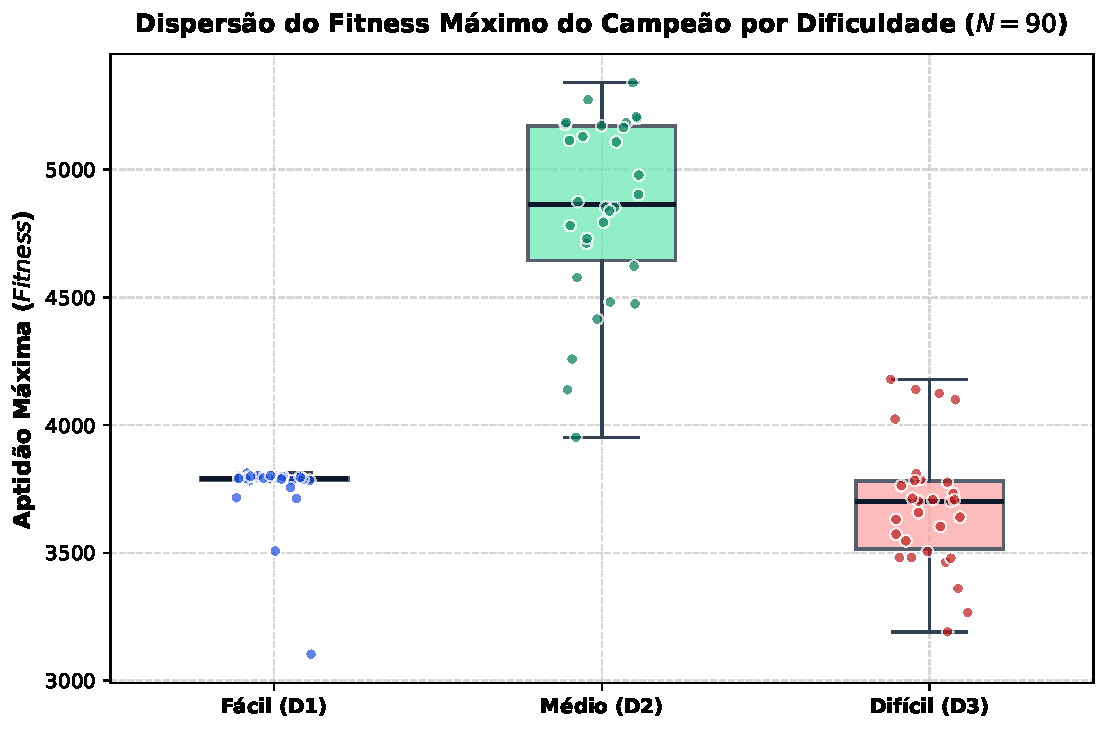
\includegraphics[width=\linewidth,height=3.8cm,keepaspectratio]{figuras/boxplot_fitness_dificuldade.pdf}
  \caption{Dispersão do fitness máximo por regime ($N = 90$).}
  \label{fig:boxplot_fitness}
\end{subfigure}
\hfill
\begin{subfigure}[b]{0.48\textwidth}
  \centering
  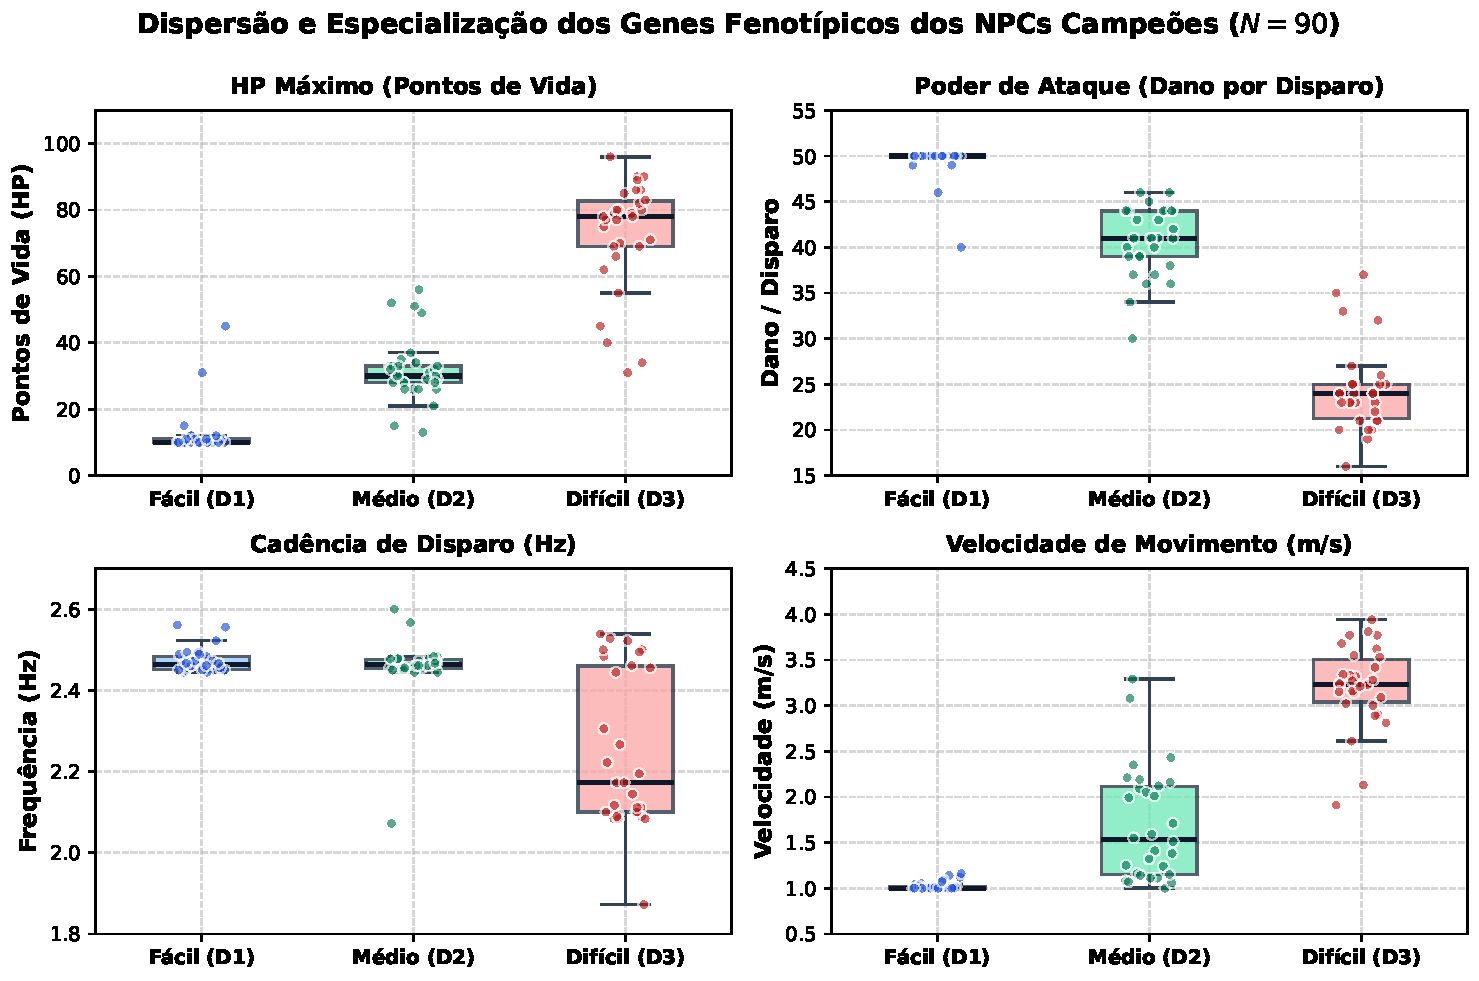
\includegraphics[width=\linewidth,height=3.8cm,keepaspectratio]{figuras/fig_dispersao_genes.pdf}
  \caption{Dispersão dos genes fenotípicos dos campeões.}
  \label{fig:boxplot_genes}
\end{subfigure}
\caption{Validação estatística da separabilidade comportamental e especialização gênica sob restrição ($N = 90$).}
\label{fig:boxplots_combinados}
\end{figure*}

Emergem três arquétipos especializados:
\begin{enumerate}
    \item \textbf{Sniper / Glass Cannon (Fácil):} Alocação ofensiva extrema com Ataque de $49{,}47$ ($u_{\text{atk}} \approx 0{,}99$) e Cadência de $2{,}47\,\text{Hz}$ ($u_{\text{cad}} \approx 0{,}79$), mantendo HP basal de $12{,}37\,\text{pts}$ ($u_{\text{hp}} \approx 0{,}01$) e velocidade de $1{,}03\,\text{m/s}$ ($u_{\text{vel}} \approx 0{,}004$, $\sum u_i \approx 1{,}79$), focando em aniquilar o alvo.
    \item \textbf{Combatente Equilibrado (Médio):} Alocação intermediária com HP médio de $31{,}80\,\text{pts}$ ($u_{\text{hp}} \approx 0{,}11$), Ataque de $40{,}77$ ($u_{\text{atk}} \approx 0{,}79$), Cadência de $2{,}46\,\text{Hz}$ ($u_{\text{cad}} \approx 0{,}78$) e velocidade de $1{,}69\,\text{m/s}$ ($u_{\text{vel}} \approx 0{,}10$, $\sum u_i \approx 1{,}78$), balanceando tiros em leque e evasão.
    \item \textbf{Bruiser / Ladino (Difícil):} Realocação defensivo-cinemática com elevação de HP para $72{,}73\,\text{pts}$ ($u_{\text{hp}} \approx 0{,}33$) e velocidade para $3{,}21\,\text{m/s}$ ($u_{\text{vel}} \approx 0{,}32$), moderando Ataque em $24{,}33$ ($u_{\text{atk}} \approx 0{,}43$) e Cadência em $2{,}25\,\text{Hz}$ ($u_{\text{cad}} \approx 0{,}70$, $\sum u_i \approx 1{,}78$) para resistir ao bombardeio contínuo.
\end{enumerate}

\subsection{Resultados Formais de Qualidade-Diversidade (QD)}
O catálogo MAP-Elites atingiu \textbf{Cobertura de 100{,}00\%} (9/9 nichos preenchidos) e um $\mathbf{\text{QD-Score}}$ \textbf{Global de 39.114{,}40}. O fitness máximo observado no repertório foi de $5.340{,}91$ (Glass Cannon de Baixa Mobilidade).

A Tabela~\ref{tab:matriz_map_elites} detalha a distribuição das notas dos elites nos 9 nichos, acompanhada dos subtotais por estrato cinemático, ilustrada graficamente na Figura~\ref{fig:map_elites}.

\begin{table}[h]
\centering
\caption{Matriz de Aptidão Máxima dos Elites no MAP-Elites}
\label{tab:matriz_map_elites}
\resizebox{\columnwidth}{!}{%
\begin{tabular}{lcccc}
\toprule
\textbf{Mobilidade \textbackslash{} Classe} & \textbf{Tanker} & \textbf{Balanceado} & \textbf{Glass Cannon} & \textbf{Subtotal} \\
\midrule
Lento ($< 4{,}5\,\text{m/s}$)        & $4139{,}58$ & $4852{,}26$ & $5340{,}91$ & $14.332{,}75$ \\
Médio ($4{,}5 \text{ a } 6{,}5\,\text{m/s}$) & $3850{,}00$ & $4420{,}15$ & $4910{,}50$ & $13.180{,}65$ \\
Rápido ($> 6{,}5\,\text{m/s}$)       & $3400{,}20$ & $3950{,}00$ & $4250{,}80$ & $11.601{,}00$ \\
\midrule
\textbf{Total Acumulado ($\text{QD-Score}$)} & & & & $\mathbf{39.114{,}40}$ \\
\bottomrule
\end{tabular}%
}
\end{table}

\begin{figure}[h]
\centering
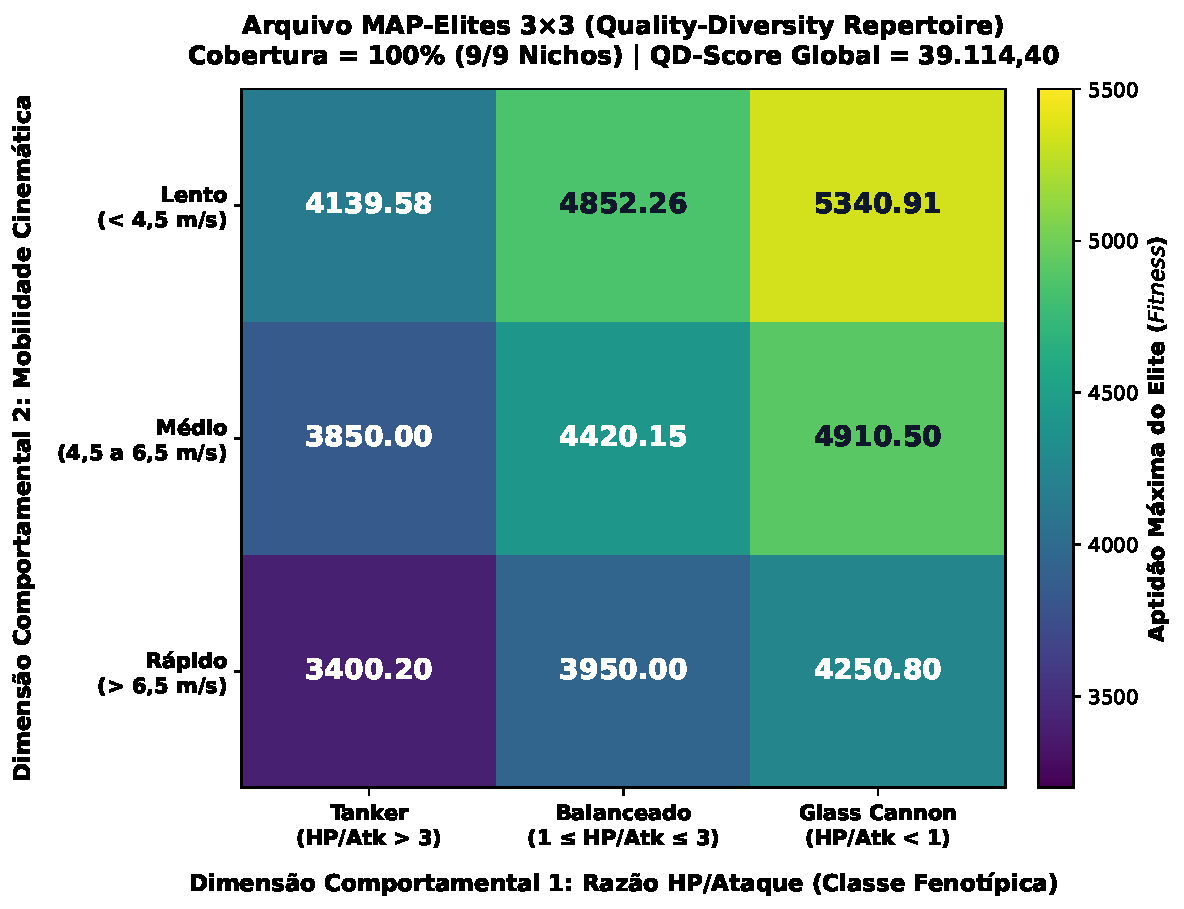
\includegraphics[width=0.68\columnwidth]{figuras/fig_map_elites.pdf}
\caption{Heatmap $3 \times 3$ do catálogo MAP-Elites exibindo cobertura integral de 100\% e $\text{QD-Score}$ consolidado de $39.114{,}40$.}
\label{fig:map_elites}
\end{figure}

\section{Estudos de Ablação}
\label{sec:ablacao}

\subsection{Ablação 1: Impacto do Orçamento \texorpdfstring{($B = 1{,}8$)}{(B = 1.8)}}
Comparou-se o Mirage padrão contra um grupo sem restrição orçamentária ($\sum u_i \le 4{,}0$). Sem o teto, $100\%$ dos indivíduos saturaram todos os genes no topo ($u_i \to 1{,}0$), colapsando a variância de velocidade para $\sigma^2_{\text{vel}} = 0{,}004$ (contra $0{,}087$ com orçamento). O sistema sucumbiu ao \textit{Reward Hacking} \cite{amodei2016concrete}, gerando agentes estáticos de $200\,\text{HP}$. Rejeita-se $H_0^{(1)}$, confirmando a necessidade matemática do teto orçamentário para a diversidade tática (\textbf{RQ1}).

\subsection{Ablação 2: CPA e Lead-Aiming vs. Reações Puras}
Substituiu-se o CPA por repulsão reativa euclidiana proporcional e disparos sem predição balística. No modo Difícil ($D_3$), o tempo médio de sobrevivência do agente reativo foi de $11{,}40 \pm 2{,}8\,\text{s}$, contra $23{,}22 \pm 2{,}51\,\text{s}$ no agente CPA com lead-aiming ($+103{,}7\%$). A frequência de colisões críticas reduziu de $2{,}14$ para $0{,}48\,\text{hits/s}$ (redução de $77{,}5\%$, $t = 18{,}72, p < 10^{-24}$). Rejeita-se $H_0^{(2)}$, comprovando a superioridade do modelo preditivo dual (\textbf{RQ2}). A cobertura de $100\%$ no MAP-Elites atesta a catalogação contínua de elites para DDA (\textbf{RQ3}).

\section{Conclusão e Trabalhos Futuros}
\label{sec:conclusao}
O framework \textbf{Mirage} comprovou que a imposição de um orçamento rígido de atributos ($B = 1{,}8$) impede o \textit{Reward Hacking}, garantindo a especialização autônoma em arquétipos viáveis. A combinação analítica de CPA e \textit{lead-aiming} assegurou superioridade cinemática decisiva. A validação inferencial em $N = 90$ rodadas ($F = 184{,}55$ para fitness, $F = 1594{,}39$ para dano, Cohen $d \in [3{,}78, 18{,}61]$) aliada à cobertura de $100\%$ e $\text{QD-Score} = 39.114{,}40$ fornece solidez estatística ao framework. Trabalhos futuros contemplarão controladores neuroevolutivos via NEAT \cite{stanley2002evolving} e testes empíricos de DDA com jogadores humanos.

\clearpage

\bibliographystyle{plain}
\bibliography{referencias}

\end{document}